In questo capitolo ...

\section{Architettura e tecnologie utilizzate}

\textcolor{red}{Mostrare diagramma dell'architettura e dei compiti dei singoli componenti\\
	Spiegare il perch� delle scelte architetturali\\
	Dire quali tecnologie sono state sfruttate per la realizzazione del backend}

\begin{figure}[h]
	\centering
	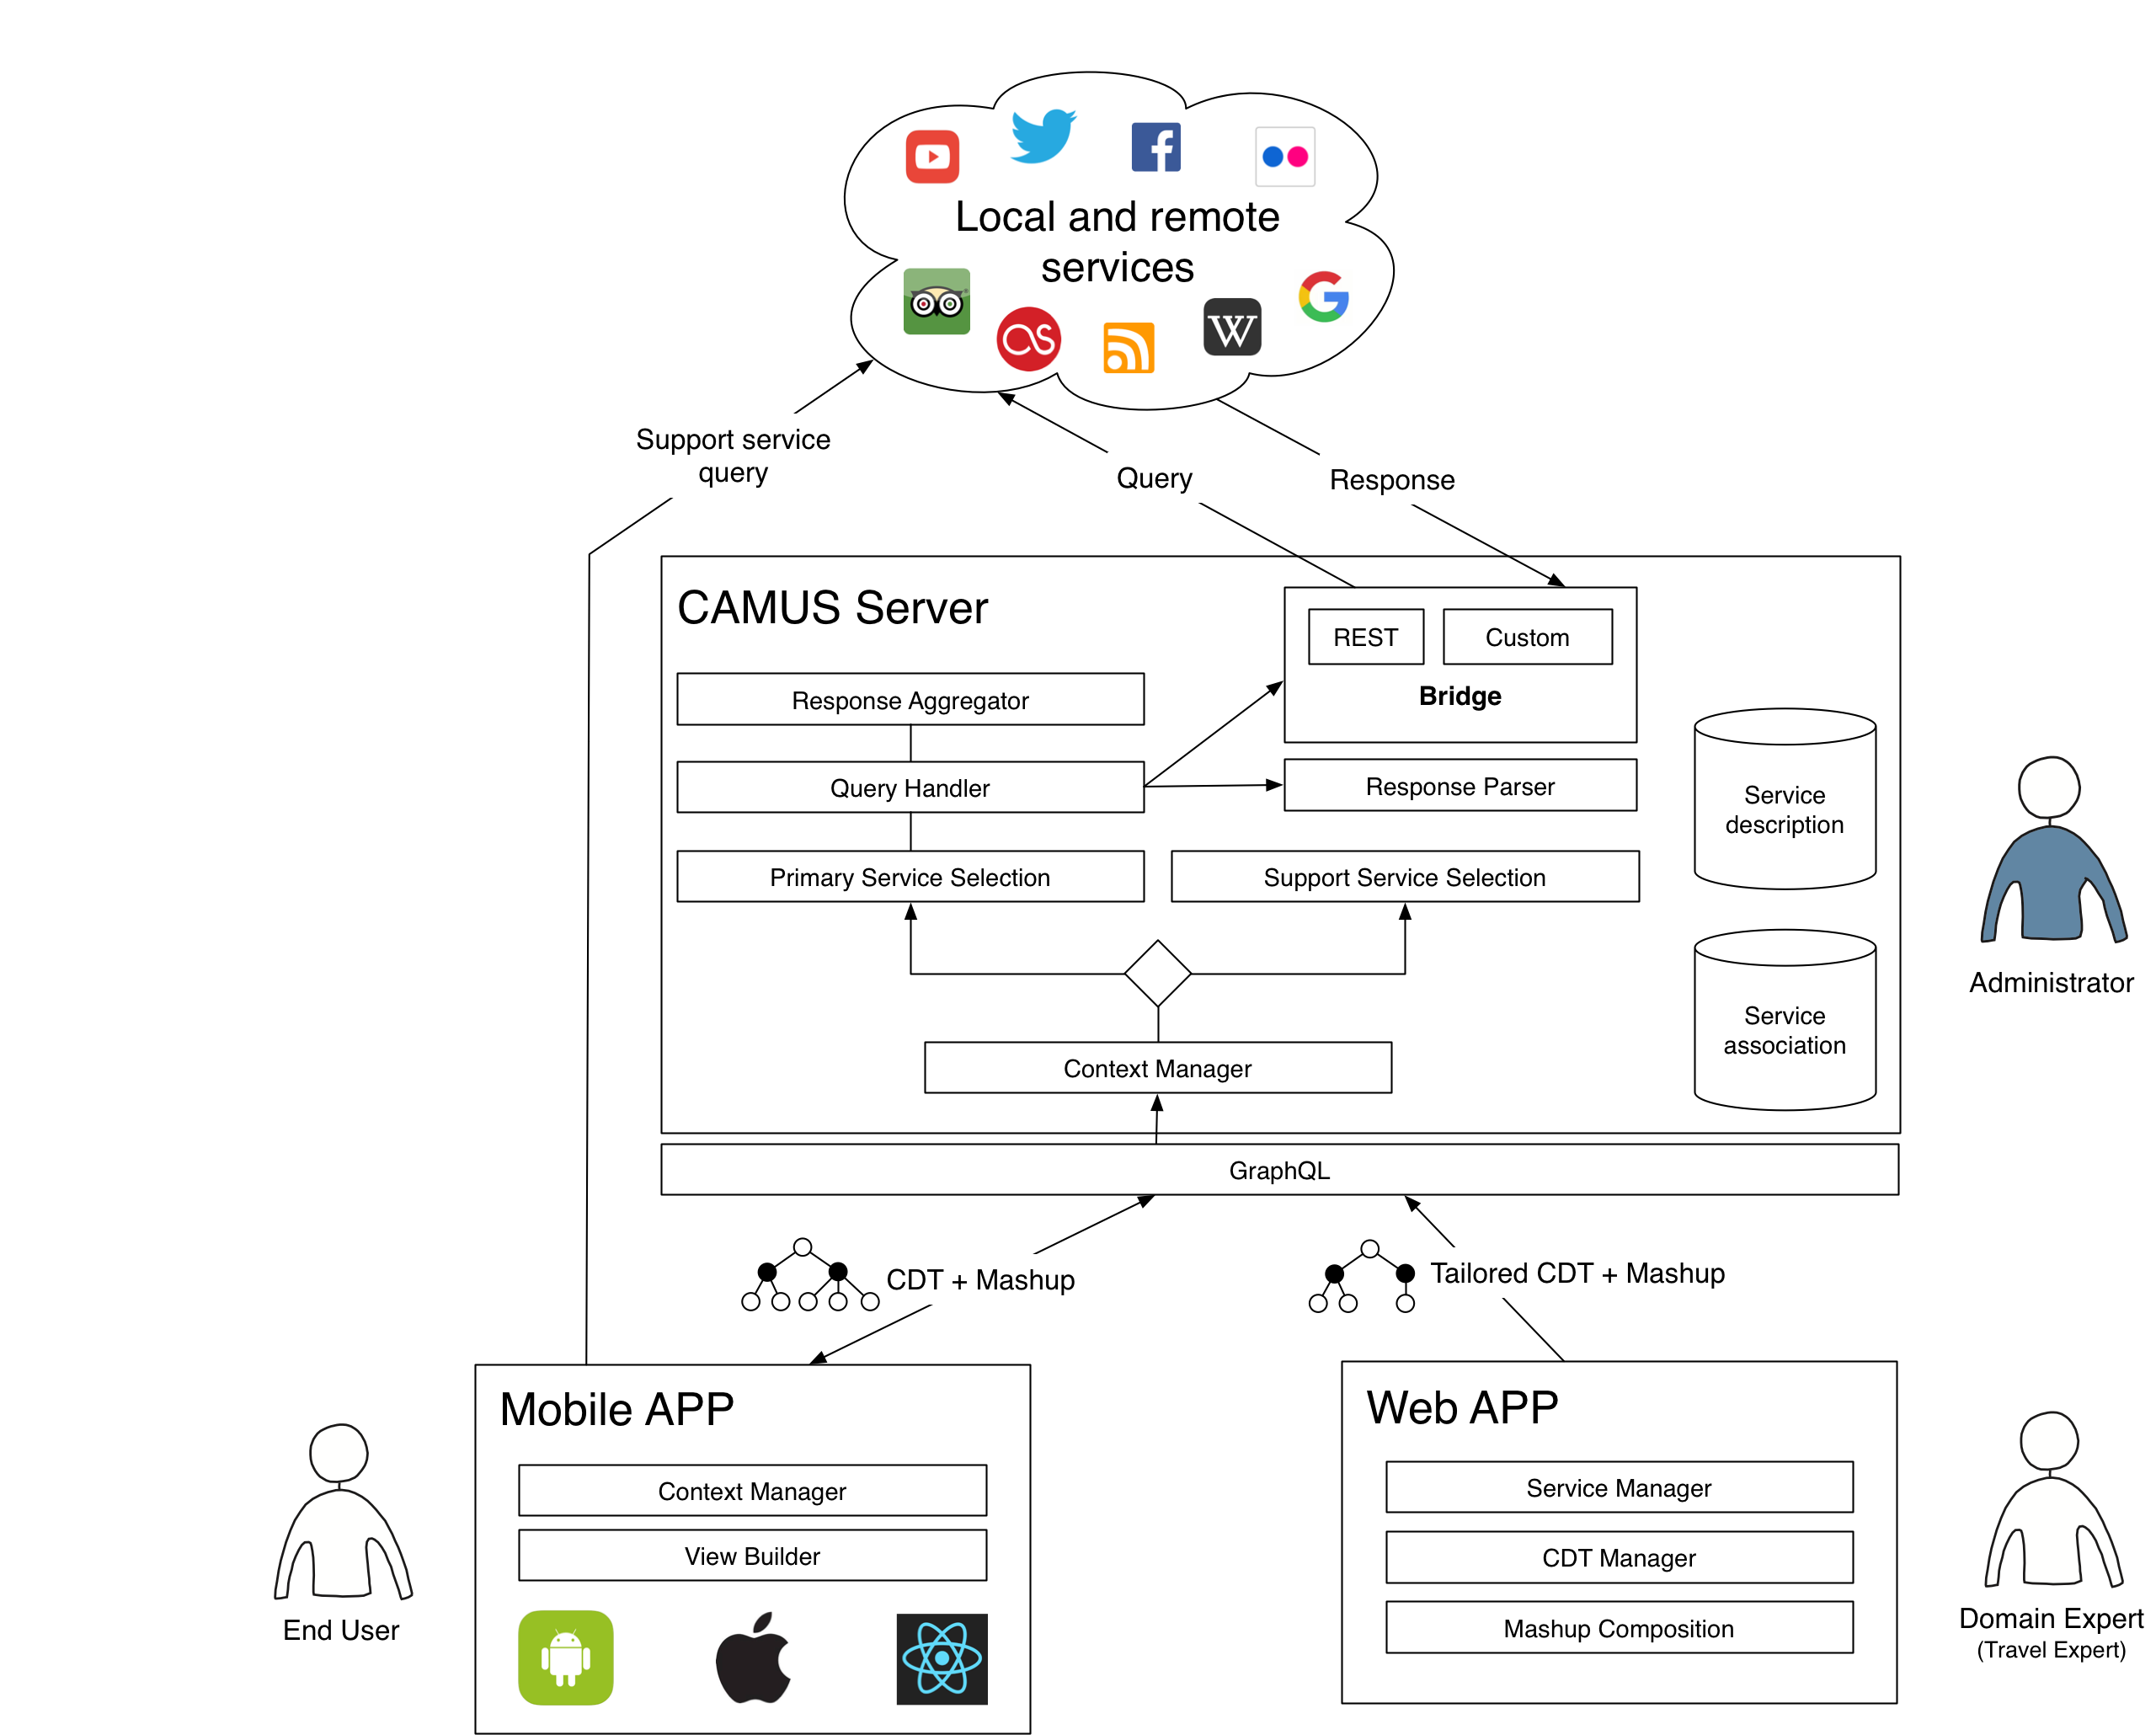
\includegraphics[width=\textwidth]{5-implementazione-backend/Immagini/camus-architecture.png}
	\caption{Architettura del backend}\label{fig:architettura-backend}
\end{figure}

\section{Descrittore dei servizi}

\textcolor{red}{Analizzare il formato del descrittore dei servizi}

In CAMUS l'acquisizione dei dati avviene tramite servizi, come descritto nella Sezione \ref{sec:utilizzo-servizi}. Affinch� il sistema possa effettuare le richieste, � necessario che sia presente una formato per descrivere le caratteristiche di ogni servizio (es.: l'indirizzo verso il quale effettuare la richiesta, i parametri da inserire, ecc.). Per questo motivo � stato introdotto l'utilizzo di un \emph{descrittore dei servizi}, che sia in grado di descrivere tutte le possibili configurazioni che i servizi possono richiedere. I \emph{descrittori} non sono altro che file JSON che specificano le impostazioni di ogni servizio. Di seguito verranno analizzati nel dettaglio tutti i campi che compongono il descrittore. Visto che il descrittore contiene una moltitudine di informazioni che riguardano diversi aspetti di un servizio, viene diviso in sotto-oggetti in modo da semplificarne la comprensione e lettura.

\subsection{Oggetto principale}

\upe il punto di partenza per la descrizione di un servizio. Comprende i seguenti campi:

\begin{itemize}
	\item \textbf{Name} \upe il nome associato al servizio
	\item \textbf{Description} Fornisce una descrizione delle funzionalit� del servizio
	\item \textbf{Protocol} Definisce la tipologia con la quale accedere al servizio. Pu� assumere i valori \virgolette{rest}, \virgolette{query} o \virgolette{custom}, per specificare rispettivamente che il servizio viene invocato secondo la logica rest, viene composta una query con parametri o necessita di un metodo particolare per l'accesso
	\item \textbf{Base Path} Rappresenta l'indirizzo di base del servizio. A partire da questo indirizzo verr� composto quello completo aggiungendo in coda i percorsi specifici delle \emph{operazioni} richieste. Non deve essere aggiunta al termine nessuna slash (\virgolette{/})
	\item \textbf{Operazioni} L'elenco delle operazioni esposte dal servizio. Per un approfondimento riguardo questo oggetto fare riferimento alla Sezione \ref{sec:descrittore-operazioni}
\end{itemize}

\subsection{Operazioni\label{sec:descrittore-operazioni}}

Rappresenta le operazioni che sono messe a disposizione dal servizio. Un'operazione viene descritta come di seguito:

\begin{itemize}
	\item \textbf{Name} Il nome dell'operazione
	\item \textbf{Type} Rappresenta la tipologia dell'operazione. Un'operazione pu� essere \emph{primaria} o di \emph{supporto}. Questa distinzione viene utilizzata principalmente per permettere la catalogazione delle operazioni da mostrare nelle web app
	\item \textbf{Description} La descrizione dell'attivit� svolta dall'operazione
	\item \textbf{Path} Il percorso specifico per richiamare l'operazione. Questo valore viene aggiunto al \emph{Base Path} del servizio. Deve essere sempre preceduto da una slash (\virgolette{/})
	\item \textbf{Bridge Name} Questo campo � opzionale, definisce il nome del bridge con la logica necessaria per invocare il servizio. \upe obbligatorio quando per il servizio viene utilizzato il protocollo \emph{custom}
	\item \textbf{Parameters} Definisce l'elenco dei parametri accettati in input dall'operazione. Per ulteriori dettagli su questo oggetto si fa riferimento alla Sezione \ref{sec:descrittore-parametri}
	\item \textbf{Headers} In questo oggetto vengono definiti gli attributi da aggiungere all'header della richiesta. Questo oggetto viene definito nella Sezione \ref{sec:descrittore-header}
	\item \textbf{Response Mapping} Serve per definire le regole di associazione per mappare la risposta del servizio coi termini semantici utilizzati dal sistema. Maggiori dettagli sui campi di questo oggetto vengono discussi nella Sezione \ref{sec:descrittore-risposta}
	\item \textbf{Pagination} Serve a raccogliere gli attributi necessari per gestire la paginazione specifica di ogni servizio. Sono supportati meccanismi di paginazioni basati sul \emph{numero di pagina} o su \emph{token}. Questo oggetto viene analizzato nel dettaglio nella Sezione \ref{sec:descrittore-paginazione}
\end{itemize}

\subsection{Parametri\label{sec:descrittore-parametri}}

In quest'oggetto vengono definiti i parametri di input di un operazione. I parametri generalmente sono composti da un campo che ne definisce il \emph{nome} e dal rispettivo valore. In alcuni casi per� vengono accettati pi� di un valore. Il descrittore deve dunque essere in grado di gestire questa situazione. Un ulteriore compito affidato a questo oggetto � quello di acquisire il valore di un determinato parametro dal \emph{contesto}. Viene inoltre fornito un semplice sistema di traduzione dei dati acquisiti dal contesto, per permettere le trasformazioni verso un valore idoneo per l'operazione corrente. Infine, soprattutto per le operazioni di \emph{supporto}, viene permessa un'associazione del parametro verso uno o pi� \emph{termini semantici}, per permettere all'app mobile di conoscere l'attributo dove andare a recuperare il valore concreto a run-time. Nello specifico, l'oggetto � cos� composto:

\begin{itemize}
	\item \textbf{Name} Il nome del parametro. Questo campo � \emph{obbligatorio}, in quanto definisce il nome che verr� utilizzato per comporre la query per richiedere i dati
	\item \textbf{Description} La descrizione della tipologia del parametro
	\item \textbf{Required} Specifica se il parametro corrente � obbligatorio o meno in una richiesta. Non definire questo attributo equivale ad assegnargli valore \emph{false}
	\item \textbf{Type} Definisce il \emph{tipo} di dato che l'operazione si aspetta di ricevere. Le principali tipologie di dato che vengono inviate verso i servizi sono \emph{stringhe}, \emph{numeri} o \emph{date}
	\item \textbf{Default} Indica un valore predefinito per il parametro. Questo campo particolarmente utile per la web app relativa il \emph{Visual Mapping}, in quanto permette di ricevere degli esempi di risposta dai servizi da mostrare all'utente
	\item \textbf{Collection Format} Questo campo definisce il \emph{separatore} da utilizzare in caso siano presenti pi� di un valore per il parametro. Sono accettati i seguenti quattro separatori: \emph{i)} csv, comma separated values; \emph{ii)} ssv, space separated values; \emph{iii)} tsv, tab separated values; \emph{iv)} pipes. Se non specificato viene utilizzato di default il tipo \emph{csv}
	\item \textbf{Mapping CDT} Definisce uno o pi� nodi dell'albero di contesto dove andare ad acquisire il valore ricevuto dalla mobile app. Nel caso vengano associati pi� di un nodo, viene seguito l'ordine di definizione nella fase di composizione della query
	\item \textbf{Mapping Term} Definisce uno o pi� termini semantici da associare al parametro. Questi termini vengono utilizzati a run-time per andare ad acquisire il valore del parametro dalle risposte ricevute dai servizi primari
	\item \textbf{Translate} Questo oggetto viene utilizzato quando � necessario effettuare un modifica del/i valore/i acquisiti dall'albero di contesto. \upe formato dai campi \virgolette{from} e \virgolette{to}, che specificano rispettivamente il valore di \emph{origine} e quello \emph{tradotto}. Vengono definite tante traduzioni quanti sono i valori che pu� assumere il rispettivo nodo del CDT
\end{itemize}

\subsection{Header\label{sec:descrittore-header}}

Quest'oggetto definisce i campi che compongono l'header associato ad una richiesta. \upe composto dai seguenti campi:

\begin{itemize}
	\item \textbf{Name} Rappresenta il nome del campo da specificare nell'header
	\item \textbf{Value} Definisce il valore che assume il campo
\end{itemize}

\subsection{Formato della risposta\label{sec:descrittore-risposta}}

In quest'oggetto sono definite le regole con le quali vengono trasformate le risposte ricevute dal servizio nel formato interno a CAMUS, dove ogni attributo viene associato ad un rispetto \emph{termine semantico} che ne definisce il contenuto. In particolare, vengono utilizzati i seguenti campi:

\begin{itemize}
	\item \textbf{List} Definisce il l'attributo che contiene l'elenco dei risultati. \upe utile nei casi in cui la risposta, oltre ai risultati, contiene al suo interno anche dei metadati relativi l'interrogazione. Se non specificato si assume che l'elenco dei risultati incominci dalla root della risposta
	\item \textbf{Items} Vengono mappati i vari campi che compongono ogni oggetto dei risultati. In particolare vengono definiti il \virgolette{percorso} dal quale recuperare il valore ed il \virgolette{termine semantico} da associare. I campi che non vengono mappati saranno ignorati dal processo di trasformazione e le relative informazioni andranno perdute. \upe necessario dunque effettuare l'operazione di mapping delle risposte con attenzione, in modo da garantire la gestione di risposte complete
	\item \textbf{Functions} Viene permesso l'utilizzo di funzioni specifiche per trasformare i valori. Questa funzione riceve in ingresso il parametro \virgolette{value}, che rappresenta il valore corrente del campo, e deve restituire il nuovo valore che verr� sostituito a quello originale. Oltre alla funzione specifica, � necessario definire anche l'\emph{attributo} sul quale eseguire questa trasformazione. L'attributo equivale al \emph{termine semantico} definito nel punto precedente
\end{itemize}

\subsection{Paginazione\label{sec:descrittore-paginazione}}

In quest'oggetto vengono gli attributi necessari per gestire la paginazione delle risposte. In particolare il sistema � in grado di gestire due tecniche di paginazione, quella basata sul \emph{numero di pagina} e quella che utilizza dei \emph{token} per richiamare le pagine. L'oggetto � composto dai seguenti campi:

\begin{itemize}
	\item \textbf{Attribute Name} Specifica il nome del parametro da aggiungere alla query per richiamare una specifica pagina
	\item \textbf{Type} Definisce il meccanismo di paginazione da utilizzare. Sono ammessi due valori: \virgolette{number} per la paginazione basata sul numero di pagine e \virgolette{token}, per quella che sfrutta i token per richiamare le pagine successive
	\item \textbf{Token Attribute} Serve per definire dove andare a leggere nella risposta il token relativo alla pagina successiva
	\item \textbf{Page Count Attribute} Definisce l'attributo che fornisce l'informazione del numero di pagine totale che possono essere richieste
\end{itemize}

\section{Schema del database}

\textcolor{red}{fare uno schema (ER?) del database}

\section{Componenti}

\textcolor{red}{mettere in risalto l'elevata modularit� del sistema e la totale mancanza dello stato da gestire}

\subsection{Context Manager}

\textcolor{red}{spiegare quali compiti svolge il context manager}

\subsection{Primary Service Selection}

\textcolor{red}{spiegare quale compito svolge il pss, riferimento alla formula usata nel capitolo delle metodologie}

\subsection{Query Handler}

\textcolor{red}{spiegare come funziona il query handler ed interazione coi bridge}

\subsection{Bridge}

\textcolor{red}{spiegare perch� si � adottata la soluzione di un bridge generico}

\subsubsection*{REST Bridge}

\textcolor{red}{descrivere come funziona il bridge per i servizi REST}

\subsection{Response Aggregator}

\textcolor{red}{spiegare come funziona il response aggregator, riferendosi all'algoritmo descritto nel capitolo delle metodologie}

\subsection{Support Service Selection}

\textcolor{red}{spiegare come funziona la selezione dei servizi di supporto, riferendosi al capitolo delle metodologie}

\section{Endpoint GraphQL}

\textcolor{red}{Mostrare quali endpoint sono stati realizzati\\
	Accennare alcuni dettagli sul come sono stati realizzati gli schemi GraphQL\\
	Descrivere vantaggi e problematiche}

\section{Flusso di una richiesta}

\textcolor{red}{mostrare come viene elaborata una richiesta proveniente dalla mobile app\\
	mettere bene in risalto i vari passaggi}

\begin{figure}[h]
	\centering
	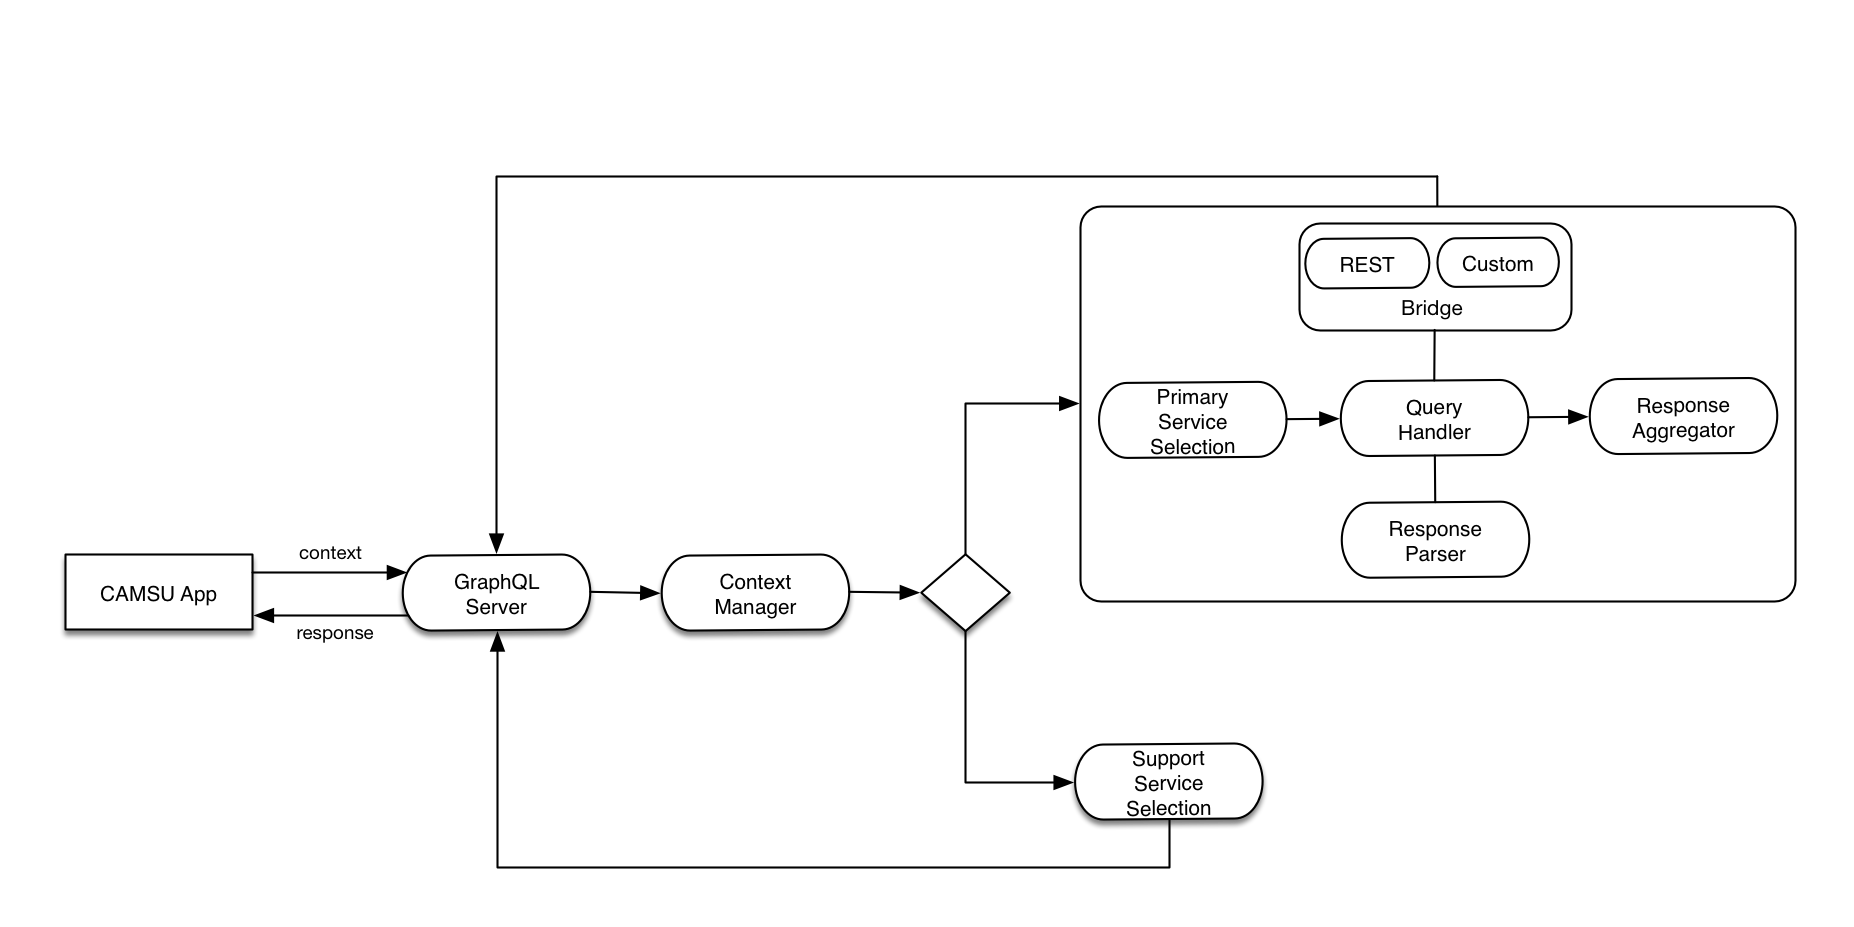
\includegraphics[width=\textwidth]{5-implementazione-backend/Immagini/camus_server_flow.png}
	\caption{Flusso di una richiesta}\label{fig:flusso-richiesta}
\end{figure}

\section{Caching dei risultati}

\textcolor{red}{Spiegare dove viene sfruttata la cache (per le risposte dei servizi e per mantenere informazioni sulla sessione)}